\documentclass[11pt,a4paper]{article}

\usepackage[a4paper,top=2.5cm,bottom=2.5cm,left=2cm,right=2cm]{geometry}
\usepackage[T1]{fontenc}
\usepackage[utf8]{inputenc}
\usepackage[scaled=0.95]{helvet}
\renewcommand{\familydefault}{\sfdefault}

\usepackage{graphicx}
\usepackage{booktabs}
\usepackage{tabularx}
\usepackage{array}
\usepackage{longtable}
\usepackage{float}
\usepackage[table]{xcolor}
\definecolor{riskgreen}{HTML}{00B050}
\definecolor{riskyellow}{HTML}{FFFF00}
\definecolor{riskorange}{HTML}{FFC000}
\definecolor{riskred}{HTML}{FF0000}
\usepackage{caption}
\usepackage{enumitem}
\usepackage{xurl}
\usepackage{cite}
\usepackage[hidelinks]{hyperref}
\usepackage{titlesec}
\usepackage{makecell}
\usepackage{chngcntr}

\counterwithin{table}{section}
\counterwithin{figure}{section}

\captionsetup{font=small,labelfont=bf}
\setlength{\parindent}{0pt}
\setlength{\parskip}{0.55em}
\setlist{nosep,leftmargin=*}
\renewcommand{\arraystretch}{1.12}
\sloppy
\raggedbottom

\titleformat{\section}{\Large\bfseries}{\thesection}{0.7em}{}
\titleformat{\subsection}{\large\bfseries}{\thesubsection}{0.6em}{}

\newcolumntype{Y}{>{\raggedright\arraybackslash}X}
\newcolumntype{L}[1]{>{\raggedright\arraybackslash}p{#1}}
\newcommand{\placeholder}[1]{\textcolor{gray}{#1}}

\makeatletter
\providecommand{\bstctlcite}[1]{%
  \@bsphack
  \@for\@citeb:=#1\do{%
    \edef\@citeb{\expandafter\@firstofone\@citeb}%
    \if@filesw\immediate\write\@auxout{\string\citation{\@citeb}}\fi
  }%
  \@esphack}
\makeatother

\begin{document}
\bstctlcite{IEEEcontrol}

\begin{titlepage}
    \centering
    \vspace*{1cm}
    {\large [Insert Institution / School / Department]\par}
    \vspace{1.5cm}
    {\Huge\bfseries Modular E-Paper Advertising Screen\par}
    \vspace{0.4cm}
    {\Large Market Opportunity and Supply Chain Strategy Template\par}
    \vspace{1.5cm}
    \begin{tabular}{@{}ll@{}}
        Unit: & [Insert Unit Code] -- [Insert Unit Name] \\
        Group: & [Insert Group Number] \\
        Submission date: & [Insert Submission Date] \\
        Assessable page limit: & [Insert Page Limit: e.g. 25 pages for five members, 30 for six] \\
        Prepared by: & [Insert team member names and student numbers] \\
    \end{tabular}
    \vfill
    \textbf{Confidentiality note:} [Insert confidentiality/NDA statement if required]

    \vspace{0.7cm}
    Project-specific content, product names, market data and claims should be inserted by the authors and supported by cited evidence.
\end{titlepage}

\pagenumbering{roman}

\section*{Workshare Declaration}
\addcontentsline{toc}{section}{Workshare Declaration}
Each main section must identify its author or co-authors. Replace the placeholders below with the agreed workshare and keep the signed version with the project logbook if required.

\begin{table}[H]
\centering
\caption{Workshare declaration template}
\footnotesize
\begin{tabularx}{\textwidth}{L{4.4cm}Y Y L{2cm}}
\toprule
\textbf{Report section} & \textbf{Author(s)} & \textbf{Evidence / files produced} & \textbf{Sign-off} \\
\midrule
Executive Summary & [Name(s)] & [Draft file / notes] & [Initials] \\
Opportunity and Market Analysis & [Name(s)] & [Dataset / notes] & [Initials] \\
Product/Service Concept Design & [Name(s)] & [Concept sketch / decision matrix] & [Initials] \\
Technical Feasibility Assessment & [Name(s)] & [Calculations / prototype notes] & [Initials] \\
Product Development Plan & [Name(s)] & [WBS / Gantt / CPA] & [Initials] \\
Team Structure & [Name(s)] & [Role research] & [Initials] \\
Supply Chain Strategy & [Name(s)] & [Supplier evidence] & [Initials] \\
Data Management Strategy & [Name(s)] & [Software list / architecture] & [Initials] \\
IP Strategy & [Name(s)] & [IP search notes] & [Initials] \\
Quality Assurance Strategy \& Assessment of a Critical Component & [Name(s)] & [QA plan / standards evidence] & [Initials] \\
Risk Assessment & [Name(s)] & [Risk register] & [Initials] \\
Sustainability and Ethics Assessment & [Name(s)] & [Ethics/sustainability evidence] & [Initials] \\
Development Budget Estimate & [Name(s)] & [Cost model] & [Initials] \\
Conclusions & [Name(s)] & [Final synthesis] & [Initials] \\
\bottomrule
\end{tabularx}
\end{table}

\tableofcontents
\clearpage
\pagenumbering{arabic}

\section{Executive Summary}
\textit{Section author(s): [Insert author(s)]}

\placeholder{[Write one or two concise paragraphs. State the societal need, the target market or user group, the proposed product/service, the core value proposition, the estimated investment requirement and the recommended decision. Avoid detailed technical explanations here.]}

\textbf{Decision requested:} \placeholder{[e.g. approve seed funding for prototype development / approve PoC build / proceed to pilot.]}

\section{Opportunity and Market Analysis}
\textit{Section author(s): Hao Yu}

The proposed modular e-paper advertising screen is aimed at a segment of the UK digital out-of-home (DOOH) advertising market suitable for poster-style, static, or low-dynamic-content delivery. It is not positioned as an alternative to all video-led screens. Instead, the concept offers lower ongoing power consumption, less light nuisance, and fewer recurring maintenance requirements compared with printed or backlit poster systems through remote content updating \cite{ref1,ref2,ref3}.

\subsection{Macro-environment, Demand and Conservative Market Sizing}

\begin{table}[H]
\centering
\caption{PESTEL summary with integrated market-demand evidence}
\scriptsize
\renewcommand{\arraystretch}{1.08}
\begin{tabularx}{\textwidth}{L{1.85cm}Y Y}
\toprule
\textbf{Factor} & \textbf{Evidence} & \textbf{Implication for the concept} \\
\midrule
Political & UK roadside advertising assets are typically managed through franchising and public-realm partnerships; local authorities can tighten operating hours, product categories and environmental conditions \cite{ref1}. & The route to market should be predominantly B2B and channel-driven, working with media operators, venues and property management teams rather than direct mass sales. \\
\addlinespace[1mm]
Economic & UK OOH revenues reach \pounds{}1.44bn by 2025, with DOOH accounting for 67\% of annual revenues \cite{ref4}. By Q3 2025, there will be 41,028 digital screen spaces in the UK \cite{ref5}. The UK business events market is valued at \pounds{}33.6bn in 2024, including 1,145 exhibitions, trade shows and conferences with exhibition space \cite{ref6}. & The demand base already exists. A phased entry strategy could start indoors before moving into selected roadside poster stock. \\
\addlinespace[1mm]
Social & Shared public spaces and venue spaces are increasingly focusing on reusable, rapidly renewable communication vehicles; night-time light control remains an operational issue in public environments \cite{ref1,ref6}. & A paper-like, lower-glare display is better aligned with wayfinding, venue communications and planning-sensitive locations than high-impact video media. \\
\addlinespace[1mm]
Technological & E Ink states that no power is needed to hold an image after it has been updated \cite{ref2}. Commercial e-paper products already exist, but mainly as indoor signage or passenger information systems rather than as a UK-standard 6-sheet advertising product \cite{ref7,ref8}. & Technical feasibility has been proven, but there remains a product gap for a modular, repairable poster-format advertising system. \\
\addlinespace[1mm]
Environmental & A Lewisham public-sector sample reports 4,062 kWh/year for a digital screen versus 1,040 kWh/year for a backlit panel, and notes that replacing scrolling 6-sheet units avoids two-weekly servicing, equivalent to 24 visits per year \cite{ref1}. & The value proposition should be sold on lifecycle performance: lower energy use, fewer service visits, and less repeated print waste. \\
\addlinespace[1mm]
Legal & UK roadside planning guidance treats these displays as poster-style media: static images should not change more frequently than every five seconds, and moving-image use is more tightly controlled \cite{ref3}. & The most defensible applications are static, poster-style advertising, wayfinding and public-information use cases rather than motion-rich campaigns. \\
\bottomrule
\end{tabularx}
\end{table}

Taken together, these conditions point to a specific sub-segment rather than a mass-market replacement play: places where buyers want remote content control but do not need full-motion video.

\begin{table}[H]
\centering
\caption{Conservative market sizing for the modular e-paper poster system}
\footnotesize
\begin{tabularx}{\textwidth}{Y L{4.4cm} L{2.8cm}}
\toprule
\textbf{Market level} & \textbf{Basis of estimate} & \textbf{Result} \\
\midrule
UK TAM: low-refresh DOOH-suitable frames & 41,028 $\times$ 30\% & 12,308 units \\
UK SAM: roadside 6-sheet style inventory & 13,733 $\times$ 60\% $\times$ 80\% & 6,592 units \\
UK SAM: indoor event poster fleet in simultaneous use & 1,145 events $\times$ 3 days $\div$ 365 $\times$ 80 displays & 753 units \\
Indicative first-year obtainable market & 2 outdoor pilot units + 60 indoor units & 62 units \\
\bottomrule
\end{tabularx}
\end{table}

\textit{Note: the 30\% parameter is an addressable-market scenario assumption, not a published industry statistic; it is used here as a conservative planning proxy informed by UK roadside display rules \cite{ref3,ref5,ref6}.}

\subsection{Competitive Position and SWOT Analysis}

\begin{table}[H]
\centering
\caption{SWOT analysis of the proposed competitive position}
\scriptsize
\renewcommand{\arraystretch}{1.08}
\begin{tabularx}{\textwidth}{Y Y}
\toprule
\textbf{Strengths} & \textbf{Weaknesses} \\
\midrule
Static content operates with very low energy consumption, has lower glare and light nuisance, supports remote updating, and has modular repairability. The concept sits between paper posters and self-illuminated DOOH rather than competing head-to-head with both \cite{ref1,ref2}. & Limited applicability to video-led campaigns; weaker colour and refresh performance; outdoor 6-sheet implementations are not yet standardised. Current outdoor e-paper prices are likely to be close to traditional outdoor digital signage \cite{ref7,ref8,ref9}. \\
\midrule
\textbf{Opportunities} & \textbf{Threats} \\
\midrule
The UK DOOH base is already large and highly digitised \cite{ref4,ref5}. Indoor events offer a much lower-risk start-up segment \cite{ref6}. Large operators such as JCDecaux and BT/Global control assets that can act as pilot host parties or channel partners rather than only competitors \cite{ref10,ref11}. & Existing operators control many premium spots \cite{ref10,ref11}. Paper posters remain cheap at point of purchase \cite{ref12}. Self-illuminated screens retain an advantage where brightness and dynamic content are critical; incumbent e-paper vendors may also move into larger advertising formats \cite{ref7,ref8,ref9}. \\
\bottomrule
\end{tabularx}
\end{table}

\begin{table}[H]
\centering
\caption{Current public price anchors for competing formats}
\footnotesize
\begin{tabularx}{\textwidth}{Y L{5.2cm}}
\toprule
\textbf{Product / format} & \textbf{Public price sample} \\
\midrule
Printed 6-sheet poster & From \pounds{}30.90 incl. VAT \cite{ref12} \\
Samsung EM32DX 32-inch e-paper display & \pounds{}958.83 ex. VAT \cite{ref7} \\
Papercast 32--42 inch outdoor e-paper display & \pounds{}4,773--\pounds{}9,817 \cite{ref8} \\
Papercast CMS licence & \pounds{}209 per display per year \cite{ref8} \\
Luminati outdoor digital poster display & \pounds{}5,185.71 ex. VAT \cite{ref9} \\
\bottomrule
\end{tabularx}
\end{table}

Price evidence suggests that outdoor e-paper is not a low-CAPEX alternative to print. The business logic therefore depends on total lifecycle cost of ownership: fewer print-and-service cycles than paper posters, lower ongoing power consumption than self-illuminated screens, and better suitability for planning-sensitive or sustainability-oriented sites \cite{ref1,ref2,ref8,ref9}.

\subsection{Customer Groups and Indicative User Personas}

The most realistic customer base is business-to-business rather than individual advertisers purchasing single screens. The concept serves a set of organisational buyers whose operational problems are similar, even though their settings differ.

\begin{table}[H]
\centering
\caption{Primary customer groups and indicative personas}
\scriptsize
\renewcommand{\arraystretch}{1.08}
\begin{tabularx}{\textwidth}{L{3.0cm} L{3.0cm} Y Y}
\toprule
\textbf{Customer group} & \textbf{Illustrative persona} & \textbf{Primary pain point} & \textbf{Why the concept fits} \\
\midrule
Street-furniture / OOH operator & Asset and partnerships manager responsible for 6-sheet or roadside inventory. & Needs remote updates, lower operating cost, reduced complaints and a credible pilot for sustainability-sensitive locations. & Useful for poster-style, lower-motion inventory where a full emissive screen may be unnecessarily energy-intensive or planning-sensitive. \\
Venue / exhibition operator & Venue operations manager or exhibitions commercial lead. & Needs reusable sponsor, programme and wayfinding displays that can be changed quickly without repeated print runs. & Indoor poster-format e-paper provides a practical proof-of-concept market with faster feedback cycles and lower deployment complexity. \\
Public-sector, campus or estate communications team & Estates and communications lead for a council, university, hospital or transport interchange. & Needs legible, low-glare information displays that support sustainability reporting and are acceptable in shared public environments. & The paper-like appearance, lower light nuisance and lower operating intensity fit governance-led procurement better than high-brightness video screens. \\
\bottomrule
\end{tabularx}
\end{table}

Overall, this market opportunity is credible because it targets a real gap between two proven solution types. UK spending on digital OOH is already high, but a significant proportion of inventory and event signage still resembles poster media more than video media \cite{ref3,ref4,ref5,ref6}. Therefore, the lowest-risk entry point should be indoor poster deployment, followed by outdoor 6-sheet pilots in locations where energy, maintenance and light-control constraints materially affect purchasing decisions \cite{ref1,ref2,ref3,ref6}.

\section{Product/Service Concept Design}
\textit{Section author(s): [Insert author(s)]}

\subsection{Concept Generation Process}
\placeholder{[Explain how the group generated alternatives. Suitable methods include brainstorming, morphological analysis, Pugh matrix, decision matrix, stakeholder mapping, or user journey analysis.]}

\subsection{Concept Selection}
\placeholder{[Explain the selection criteria and why the chosen concept is preferable. Include rejected alternatives briefly, not as a long narrative.]}

\begin{table}[H]
\centering
\caption{Concept selection matrix template}
\footnotesize
\begin{tabularx}{\textwidth}{Y L{2cm} L{2.5cm} L{2.5cm} Y}
\toprule
\textbf{Criterion} & \textbf{Weight} & \textbf{Concept A} & \textbf{Concept B} & \textbf{Rationale} \\
\midrule
Customer value & [Weight] & [Score] & [Score] & [Reason] \\
Technical feasibility & [Weight] & [Score] & [Score] & [Reason] \\
Circular economy benefit & [Weight] & [Score] & [Score] & [Reason] \\
Commercial attractiveness & [Weight] & [Score] & [Score] & [Reason] \\
\bottomrule
\end{tabularx}
\end{table}

\subsection{Selected Concept Overview}
\placeholder{[Describe the product/service architecture, user interaction, main functions and benefits. Refer to the A3 concept sketch or include a simplified system diagram.]}

\begin{figure}[H]
\centering
\fbox{\parbox{0.85\textwidth}{\centering\vspace{1.5cm}[Insert concept diagram, system architecture, CAD render or service blueprint here.]\vspace{1.5cm}}}
\caption{Concept overview placeholder}
\end{figure}

\section{Technical Feasibility Assessment}
\textit{Section author(s): [Insert author(s)]}

\subsection{Key Technical Questions}
\placeholder{[List the aspects that must be technically feasible for the concept to work, such as energy, force, data rate, mechanical load, sensor accuracy, manufacturability, reliability or safety.]}

\subsection{Feasibility Calculations and Evidence}
\placeholder{[Show calculations clearly. State assumptions, equations, units and sources. Include early prototypes, simulations or physical reasoning where relevant.]}

\begin{table}[H]
\centering
\caption{Technical feasibility calculation template}
\footnotesize
\begin{tabularx}{\textwidth}{Y Y L{3cm} L{3cm}}
\toprule
\textbf{Requirement} & \textbf{Calculation / evidence} & \textbf{Result} & \textbf{Decision} \\
\midrule
{}[Requirement 1] & [Equation, data, prototype evidence] & [Result with units] & [Pass / R\&D needed] \\
{}[Requirement 2] & [Equation, data, prototype evidence] & [Result with units] & [Pass / R\&D needed] \\
{}[Requirement 3] & [Equation, data, prototype evidence] & [Result with units] & [Pass / R\&D needed] \\
\bottomrule
\end{tabularx}
\end{table}

\subsection{Feasibility Risks and R\&D Requirements}
\placeholder{[Identify what is proven, what is uncertain and what must be tested during PoC development.]}

\section{Product Development Plan}
\textit{Section author(s): [Insert author(s)]}

\subsection{Development Strategy}
\placeholder{[Explain the development model, prototype objective, prototype success criteria and development logic.]}

\subsection{Work Breakdown Structure}
\placeholder{[Insert WBS or list major work packages: product design, software, manufacturing, testing, regulatory review, user trial, supplier qualification, etc.]}

\begin{table}[H]
\centering
\caption{Work breakdown structure template}
\footnotesize
\begin{tabularx}{\textwidth}{L{2cm}Y L{3cm}Y}
\toprule
\textbf{WBS ID} & \textbf{Task / deliverable} & \textbf{Owner} & \textbf{Dependency} \\
\midrule
1.0 & [Task] & [Role/name] & [Dependency] \\
2.0 & [Task] & [Role/name] & [Dependency] \\
3.0 & [Task] & [Role/name] & [Dependency] \\
\bottomrule
\end{tabularx}
\end{table}

\subsection{Indicative Gantt Chart}
\placeholder{[Replace the placeholder Gantt chart with the actual schedule. Keep it legible; use landscape orientation if necessary.]}

\begin{table}[H]
\centering
\caption{Gantt chart schedule template}
\footnotesize
\begin{tabularx}{\textwidth}{Y L{3cm} L{3cm}Y}
\toprule
\textbf{Work package} & \textbf{Start week} & \textbf{End week} & \textbf{Deliverable / dependency} \\
\midrule
{}[WP1] & [Week] & [Week] & [Deliverable and dependency] \\
{}[WP2] & [Week] & [Week] & [Deliverable and dependency] \\
{}[WP3] & [Week] & [Week] & [Deliverable and dependency] \\
{}[WP4] & [Week] & [Week] & [Deliverable and dependency] \\
\bottomrule
\end{tabularx}
\end{table}

\subsection{Critical Path and Milestones}
\placeholder{[Identify critical dependencies and decision gates. Add a network diagram if useful.]}

\section{Team Structure}
\textit{Section author(s): [Insert author(s)]}

\placeholder{[Define the team required to develop the concept to PoC. Include roles, required knowledge/skills/experience, estimated salaries or contractor rates, and why each role is needed.]}

\begin{table}[H]
\centering
\caption{Team structure and cost template}
\footnotesize
\begin{tabularx}{\textwidth}{L{3cm}Y L{3cm}Y}
\toprule
\textbf{Role} & \textbf{Required knowledge, experience and skills} & \textbf{Estimated cost} & \textbf{Source / basis} \\
\midrule
{}[Role 1] & [Skills] & [Salary/rate] & [Source] \\
{}[Role 2] & [Skills] & [Salary/rate] & [Source] \\
{}[Role 3] & [Skills] & [Salary/rate] & [Source] \\
\bottomrule
\end{tabularx}
\end{table}

\clearpage
\section{Supply Chain Strategy}
\textit{Section author(s): Hao Yu}

At the PoC stage, the supply-chain objective is not the lowest ex-works unit price but a build path that is fast, legally marketable in Great Britain, quality-controlled and serviceable after sale. The indoor poster-format device remains the right first product because it validates demand and content workflow before the higher-risk outdoor 6-sheet system. The bought-in item that dominates technical risk is the e-paper display engine, so supplier selection is managed as a strategic or bottleneck decision under Kraljic logic and is gated by supplier capability, quality evidence, landed cost and compliance controls \cite{ref14,ref15,ref16,ref17,ref18,ref19,ref20}.

\begin{figure}[H]
\centering
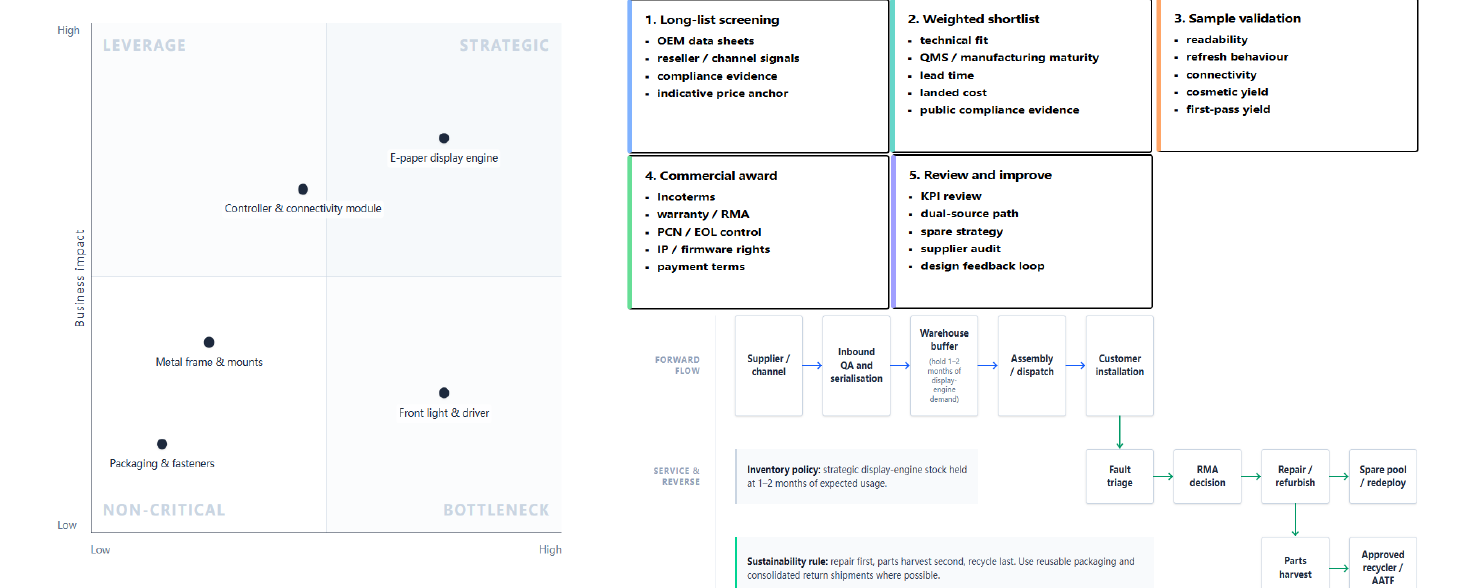
\includegraphics[width=0.98\textwidth,height=0.29\textheight,keepaspectratio]{figures/supply_chain_control_model.png}
\caption{Chart-led control model for the PoC supply chain. The supplier-selection logic follows CIPS guidance and Kraljic portfolio thinking; quality, trade and compliance gates draw on ISO 9001, Incoterms 2020 and GB product obligations \cite{ref14,ref15,ref16,ref17,ref18,ref19,ref20,ref21,ref22}.}
\end{figure}

\begin{table}[H]
\centering
\caption{Weighted shortlist example for the critical PoC component}
\label{tab:supplier-shortlist}
\footnotesize
\begin{tabularx}{\textwidth}{Y L{2.1cm} L{2.8cm} L{2.8cm}}
\toprule
\textbf{Criterion} & \textbf{Weight} & \textbf{Samsung EM32DX} & \textbf{Sharp EP-C251} \\
\midrule
Poster-format technical fit & 30\% & 5 & 3 \\
Availability / lead-time visibility & 20\% & 5 & 2 \\
Compliance evidence for GB sale & 20\% & 3 & 5 \\
Integration simplicity & 15\% & 5 & 4 \\
Indicative public price & 15\% & 5 & 4 \\
\textbf{Weighted total (/5)} & \textbf{100\%} & \textbf{4.60} & \textbf{3.55} \\
\bottomrule
\end{tabularx}
\end{table}

Scores in Table~\ref{tab:supplier-shortlist} are the project team's assessment from public specifications, reseller price signals and public conformity evidence \cite{ref23,ref24,ref25,ref26,ref27}. The recommendation is to use Samsung as the primary PoC source and Sharp as an approved second source. Samsung scores higher for poster-format fit, integration simplicity and visible delivery availability, while Sharp is stronger on publicly visible compliance documentation through its downloadable UKCA Declaration of Conformity. The recommended sourcing posture is therefore one lead supplier plus one approved fallback, not sole sourcing \cite{ref23,ref24,ref25,ref26,ref27}.

\begin{table}[H]
\centering
\caption{Commercial and legal decisions that directly affect external sourcing}
\scriptsize
\renewcommand{\arraystretch}{1.08}
\begin{tabularx}{\textwidth}{L{2.7cm}Y Y Y}
\toprule
\textbf{Decision area} & \textbf{PoC decision} & \textbf{Later-stage shift} & \textbf{Why it matters} \\
\midrule
Trading entity & Trade through a UK private company limited by shares. & Keep the Ltd entity as the contracting party for suppliers, customers and investors. & It ring-fences liability, supports inventory holding and warranties, and is more credible for B2B procurement than a sole trader \cite{ref28}. \\
Trade terms & Prefer UK stock or DDP-like simplicity even at a modest unit premium. & After design freeze, move selectively towards FCA / FOB and local final assembly of lower-risk parts. & For first builds, lead-time certainty and reduced import-admin burden are worth more than marginal ex-works savings \cite{ref17}. \\
Supplier structure & One lead display supplier plus one approved second source. & Qualify a second source formally and separate the imported display engine from locally sourced enclosures and brackets. & This reduces line-stop risk on the strategic item while allowing competitive sourcing for lower-risk parts \cite{ref14,ref15}. \\
Contract controls & Write acceptance criteria, warranty/RMA terms, PCN/EOL notice, specification control and firmware/CMS usage rights into the contract. & Add KPI review, audit rights and a minimum spare-parts support period. & The contract must protect serviceability, avoid lock-in and ensure that conformity evidence is available before GB sale \cite{ref17,ref18,ref19,ref20}. \\
\bottomrule
\end{tabularx}
\end{table}

Overall, the recommended supply chain is a phased, service-oriented model rather than a lowest-piece-price model. At PoC stage, it prioritises controllable inbound supply, 1--2 months of stock cover for the scarce display engine, and a closed-loop after-sales process that repairs and redeploys units before treating them as waste. That approach reduces launch risk, protects uptime for early customers, and improves sustainability by reducing emergency shipments, extending component life and using WEEE-compliant end-of-life routes \cite{ref17,ref21,ref22}.

\section{Data Management Strategy}
\textit{Section author(s): [Insert author(s)]}

\placeholder{[Describe the software, licences and systems required to manage design data, documentation, project controls, communication, CAD/CAE, code, manufacturing data, customer data and financial data. Include approximate licence costs.]}

\begin{table}[H]
\centering
\caption{Data management systems template}
\footnotesize
\begin{tabularx}{\textwidth}{Y Y Y L{3cm}}
\toprule
\textbf{System category} & \textbf{Example tool} & \textbf{Purpose / single source of truth} & \textbf{Estimated cost} \\
\midrule
Project management & [Tool] & [Purpose] & [Cost] \\
Documentation / collaboration & [Tool] & [Purpose] & [Cost] \\
CAD / PDM & [Tool] & [Purpose] & [Cost] \\
Code repository & [Tool] & [Purpose] & [Cost] \\
Finance / accounting & [Tool] & [Purpose] & [Cost] \\
\bottomrule
\end{tabularx}
\end{table}

\subsection{Data Security and Compliance}
\placeholder{[Identify security, access control, backup, retention and regulatory requirements. Address personal data only if the concept collects it.]}

\section{IP Strategy}
\textit{Section author(s): [Insert author(s)]}

\placeholder{[Identify IP that will be used, generated or acquired. Include patents, design rights, copyright, trademarks, trade secrets, datasets, software, brand assets and know-how. Explain protection strategy, ownership, licensing and infringement risk.]}

\begin{table}[H]
\centering
\caption{IP register template}
\footnotesize
\begin{tabularx}{\textwidth}{Y L{4cm}Y Y}
\toprule
\textbf{IP asset} & \textbf{IP type} & \textbf{Protection route} & \textbf{Owner / risk} \\
\midrule
{}[Asset 1] & [Patent/design/copyright/etc.] & [Action] & [Owner/risk] \\
{}[Asset 2] & [Patent/design/copyright/etc.] & [Action] & [Owner/risk] \\
{}[Asset 3] & [Patent/design/copyright/etc.] & [Action] & [Owner/risk] \\
\bottomrule
\end{tabularx}
\end{table}

\section{Quality Assurance Strategy \& Assessment of a Critical Component}
\textit{Section author(s): [Insert author(s)]}

\subsection{Quality Strategy}
\placeholder{[Explain how quality will be managed during design, supplier selection, manufacturing, assembly, testing and service. Include standards or legal requirements where relevant.]}

\subsection{Critical Component Assessment}
\placeholder{[Select one critical component and demonstrate the assessment process. Include requirements, supplier evidence, acceptance criteria and inspection/test plan.]}

\begin{table}[H]
\centering
\caption{Critical component quality plan template}
\footnotesize
\begin{tabularx}{\textwidth}{Y Y Y L{3cm}}
\toprule
\textbf{Requirement} & \textbf{Acceptance criterion} & \textbf{Test / inspection method} & \textbf{Responsibility} \\
\midrule
{}[Requirement 1] & [Criterion] & [Method] & [Owner] \\
{}[Requirement 2] & [Criterion] & [Method] & [Owner] \\
{}[Requirement 3] & [Criterion] & [Method] & [Owner] \\
\bottomrule
\end{tabularx}
\end{table}

\section{Risk Assessment}
\textit{Section author(s): [Xuyang Gu]}

The modular e-paper display project faces several important risks during proof-of-concept (PoC) development and early commercialisation. Because the concept depends on specialist e-paper hardware, modular assembly, software-controlled content delivery and lawful market entry, the main risks are those that could delay the PoC, weaken customer confidence, or prevent successful early deployment. The overall risk profile remains manageable, but only if the project follows a phased, indoor-first launch strategy and validates the product first in static-content applications before considering wider rollout \cite{ref6,ref2,ref4}.

\subsection{Market Adoption Risk}

Market adoption risk concerns whether the product can secure enough early demand in the most suitable pilot segments. The modular e-paper display is not intended to replace all digital advertising formats; rather, it is a specialist solution for static or low-dynamic content where lower operating intensity, lower glare and lifecycle efficiency are valued more than motion and brightness. This positioning is most credible in venues, conferences, campuses and other governance-led or public-information environments, rather than across the full DOOH market \cite{ref6}. At the same time, the broader OOH sector remains highly competitive and commercially mature, which means the product may still be compared unfavourably with cheaper printed posters or brighter LED/LCD systems if it is marketed too broadly \cite{ref4}. For this reason, early segment selection is critical.

\subsection{Technical Performance Risk}

Technical performance risk concerns whether the product can perform reliably in real operating conditions. E-paper provides clear benefits for static display use because it is bistable and therefore consumes very little power while holding an image \cite{ref2}. However, that same technology also introduces limits in refresh speed, colour responsiveness and night-time visibility, especially where front lighting is required. In addition, larger modular layouts may create visual-quality issues such as seams, alignment errors or inconsistent panel appearance. These risks do not invalidate the concept, but they do mean that the product should first be validated in poster-style applications rather than in highly demanding outdoor display environments \cite{ref2}.

\subsection{Supply-Chain and Lock-In Risk}

Supply-chain and lock-in risk concerns the project's dependence on critical suppliers and supplier-controlled platforms. The display engine is the most strategically important hardware component in the system, and supplier concentration should therefore be treated as a strategic procurement risk because it may increase exposure to delays, pricing pressure and reduced flexibility \cite{ref14,ref15}. A related issue is CMS and firmware lock-in: vendor tools may reduce development effort at PoC stage, but they may also reduce future control if the business becomes dependent on supplier-controlled workflows. For this reason, the project should maintain at least one fallback source where possible and ensure that firmware release control and content-upload capability remain under operator control \cite{ref14,ref15}.

\subsection{Compliance and Governance Risk}

Compliance and governance risk concerns whether the product can be developed and deployed in a controlled and lawful way. The system must satisfy conformity and RoHS-related obligations before sale or wider pilot use, and these requirements are not optional administrative issues but basic conditions of lawful market entry \cite{ref19,ref20}. In addition, WEEE-related responsibilities remain important for end-of-life recovery and treatment \cite{ref22}. Some intended use environments may also be planning-sensitive, particularly if the system is treated as if it were moving-image signage rather than static digital display. Governance risk further includes weak document control, poor release history and inadequate traceability of approved versions. In addition, inadequate handling of customer, supplier or service data would create further governance risk under UK GDPR requirements \cite{ref29}. These issues are especially important because weak compliance or weak governance would reduce confidence in the product even if the hardware itself performs well.

\subsection{Operational Reliability and Service Risk}

Operational reliability and service risk concerns whether the product can actually deliver the modular, repair-oriented value proposition claimed by the project. If maintenance access is slow, module replacement is difficult, or after-sales support is weak, then downtime may increase and the practical benefit of modularity may be lost. The same applies to poor service traceability: if return records, serial numbers and test history are not clearly linked, recurring faults become more difficult to diagnose and control. These risks matter because early customer perception will depend not only on display performance, but also on whether failed units can be restored quickly and predictably. WEEE-compliant recovery and treatment routes also reinforce the importance of structured return and repair processes rather than unmanaged replacement or disposal \cite{ref22}.

\subsection{Financial Risk}

Financial risk concerns whether the concept can remain commercially viable through PoC development and early rollout. The project may struggle if customers assess it only against upfront purchase cost rather than lifecycle value. This is particularly important because the product is likely to face higher early hardware costs than printed alternatives, even where it offers lower operating energy, lower service intensity and better public acceptability over time. As a result, the concept is more likely to be commercially credible in those segments where lifecycle efficiency and operational practicality already influence procurement decisions, such as business events, venues and governance-led environments \cite{ref6,ref4}. A related financial risk is that development, compliance and pilot costs may rise faster than expected before stable demand is established. For that reason, the project should prioritise controlled pilots and staged investment rather than broad expansion at an early stage.

Overall, the project's risks are manageable if the business follows a phased and controlled launch strategy. The most important risks relate to technical performance, supply-chain stability, compliance readiness and early service delivery. These do not invalidate the concept, but they do mean that the PoC should be validated first in lower-risk indoor and static-content applications before wider rollout is considered \cite{ref2}\cite{ref4}\cite{ref6}.


\textbf{Risk rating approach:}  Severity describes the consequence if the risk occurs, using the scale Negligible, Minor, Moderate, Significant and Severe. Likelihood describes the probability of occurrence, using the scale Highly unlikely, Unlikely, Possible, Likely and Very likely. In the detailed risk register, each risk was assigned a numerical likelihood score and severity score on a 1–5 scale, and the priority level was calculated as likelihood × severity. The six key risks with the highest priority levels are summarised in Table 11.1, while the full risk register is provided in Appendix A.
\begin{table}[H]
\centering
\caption{Summary risk table for PoC development and early deployment}
\label{tab:summary-risk-table}
\renewcommand{\arraystretch}{1.55}
\setlength{\tabcolsep}{5pt}
\small

\begin{tabularx}{\textwidth}{|>{\centering\arraybackslash}X|>{\centering\arraybackslash}p{1.8cm}|>{\centering\arraybackslash}X|}
\hline
\textbf{\large Key risk} &
\begin{tabular}[c]{@{}c@{}}\textbf{\large Priority}\\\textbf{\large level}\end{tabular} &
\textbf{\large Risk response} \\
\hline

Market adoption risk (Commercial) -- The product may face weaker-than-expected demand because it is only suitable for static or low-dynamic content, and may be compared unfavourably with cheaper print or brighter LED/LCD alternatives \cite{ref6,ref4}.
& 16
& Target indoor venues, exhibitions, campuses and governance-led environments first; position the system as a specialist poster-style solution sold on lifecycle value rather than pure upfront price \cite{ref6,ref4}. \\
\hline

Technical performance risk (Technical) -- Slow refresh, limited suitability for motion-rich content, night-visibility constraints and larger-scale visual-quality issues may reduce customer confidence in real operating conditions \cite{ref2}.
& 20
& Restrict early deployment to static-content applications; validate front lighting, tiled display quality, mounting and enclosure performance during PoC testing before wider rollout \cite{ref2}. \\
\hline

Supply-chain and lock-in risk (Technical / Commercial) -- Dependence on a limited supplier base and vendor-controlled CMS or firmware tools may create delays, switching costs and reduced long-term flexibility \cite{ref14,ref15}.
& 15
& Maintain one lead supplier plus one approved fallback source where possible; require standard image-upload capability and operator-controlled firmware release processes \cite{ref14,ref15}. \\
\hline

Compliance and governance risk (Compliance / Commercial) -- The product may be delayed, restricted or rejected if conformity, RoHS, WEEE, document-control or data-governance requirements are not addressed in time \cite{ref19,ref20,ref22,ref29}.
& 15
& Complete compliance evidence before sale; maintain controlled release history and approval records; and apply lawful data-handling and traceability processes \cite{ref19,ref20,ref22,ref29}. \\
\hline

Operational reliability and service risk (Technical / Project) -- Slow maintenance, weak RMA response and poor service traceability may reduce uptime and undermine the repairable business model \cite{ref2,ref22,ref29}.
& 12
& Validate quick-swap maintenance procedures; use serial traceability, spare kits and structured return-and-repair processes during pilot deployment \cite{ref2,ref22}. \\
\hline

Financial risk (Project / Financial) -- High early unit cost and rising development or compliance costs may create cash-flow pressure before stable demand is established \cite{ref6,ref4}.
& 16
& Prioritise controlled pilots and staged investment; focus on customers who value lifecycle efficiency and operational practicality rather than lowest upfront cost \cite{ref6,ref4}. \\
\hline

\end{tabularx}

\normalsize
\end{table}

Table~\ref{tab:risk-matrix} shows the distribution of the identified risks by likelihood and severity, highlighting those requiring the greatest management attention during PoC development and early deployment.
\begin{table}[H]
\centering
\caption{Risk matrix showing likelihood and severity ratings}
\label{tab:risk-matrix}
\renewcommand{\arraystretch}{1.45}
\setlength{\tabcolsep}{6pt}
\small

\begin{tabularx}{\textwidth}{|>{\bfseries\raggedright\arraybackslash}p{3.0cm}|>{\centering\arraybackslash}X|>{\centering\arraybackslash}X|>{\centering\arraybackslash}X|>{\centering\arraybackslash}X|>{\centering\arraybackslash}X|}
\hline
\textbf{Likelihood \textbackslash{} Severity} 
& \textbf{Negligible} 
& \textbf{Minor} 
& \textbf{Moderate} 
& \textbf{Significant} 
& \textbf{Severe} \\
\hline

Very likely 
& \cellcolor{riskyellow} 
& \cellcolor{riskyellow} 
& \cellcolor{riskorange} 
& \cellcolor{riskred} 
& \cellcolor{riskred} \\
\hline

Likely 
& \cellcolor{riskgreen} 
& \cellcolor{riskyellow} 
& \cellcolor{riskorange} 
& \cellcolor{riskorange}\textbf{B, G, O, Q} 
& \cellcolor{riskred}\textbf{C} \\
\hline

Possible 
& \cellcolor{riskgreen} 
& \cellcolor{riskgreen} 
& \cellcolor{riskyellow}\textbf{I, M, P} 
& \cellcolor{riskyellow}\textbf{A, E, H, K, L, N, R} 
& \cellcolor{riskorange}\textbf{D, J} \\
\hline

Unlikely 
& \cellcolor{riskgreen} 
& \cellcolor{riskgreen} 
& \cellcolor{riskyellow} 
& \cellcolor{riskyellow}\textbf{F} 
& \cellcolor{riskorange} \\
\hline

Highly unlikely 
& \cellcolor{riskgreen} 
& \cellcolor{riskgreen} 
& \cellcolor{riskgreen} 
& \cellcolor{riskyellow} 
& \cellcolor{riskyellow} \\
\hline

\end{tabularx}

\vspace{0.3em}
\footnotesize\emph{Note: A--R correspond to the detailed risks listed in Appendix. Green indicates lower priority, yellow indicates medium priority, orange indicates high priority, and red indicates critical priority.}

\normalsize
\end{table}

\section{Sustainability and Ethics Assessment}
\textit{Section author(s): [Xuyang Gu]}

The sustainability and ethics case for the modular e-paper display is strongest when assessed through a Triple Bottom Line lens: People, Planet and Profit. This is a useful framework because the project is not only trying to reduce electricity use; it also aims to improve public acceptability, support a more repair-oriented product lifecycle and create a viable commercial proposition. However, the sustainability case must remain bounded. The concept is most credible as a lower-intensity display solution for static and low-dynamic applications, not as a blanket replacement for all digital signage \cite{ref6}.

\subsection{People}

From a social perspective, the main benefit of the concept is reduced visual and operational intensity in shared environments. The intended use cases, including conference signage, venue communication, wayfinding and selected public-information displays, are all environments where readability, updateability and public acceptability often matter more than full-motion visual impact \cite{ref6}. Because e-paper is reflective rather than self-emissive, it can reduce glare and avoid the constant brightness associated with many digital displays \cite{ref2}. This gives the concept a stronger social justification than a conventional high-brightness LED screen in the same setting.

There is also a health-related argument for taking nighttime light exposure seriously. A recent systematic review concluded that artificial light at night is associated with sleep disturbance, although the authors also noted methodological limits in the evidence base \cite{ref30}. A separate study reported a significant association between higher artificial light at night exposure and increased insomnia-related social burden \cite{ref31}. These studies do not prove that replacing LED signage with e-paper will solve those problems on its own, but they do support the broader claim that reducing unnecessary nighttime light exposure is socially valuable. For that reason, a lower-glare reflective medium can be presented as a more socially responsible option where digital signage is genuinely needed.

The ethical limit, however, is clear: a lower-energy screen is not automatically socially beneficial if it is simply used to increase the volume of advertising in already saturated public spaces. The strongest ethical position is therefore substitution rather than expansion. In other words, the project is easiest to defend when it replaces more intrusive or more resource-intensive formats in places where digital communication is already justified, rather than when it is used to normalise more screen-based advertising overall.

Inclusivity should also be considered in how users interact with the display. As engineering outputs should be usable by different groups of people, the system should support clear contrast, readable typography, suitable mounting height and flexible content formatting for public-information use. This is particularly relevant in venues and wayfinding contexts, where users may differ in age, language background, visual ability and familiarity with the space. In this sense, the social case for e-paper is not only reduced glare, but also the opportunity to design a calmer and more accessible communication medium.

\subsection{Planet}

The clearest environmental advantage is lower operating energy. E Ink states that its technology needs no power to hold an image once updated \cite{ref2}. That principle makes e-paper fundamentally different from self-emissive LED signage, which consumes electricity continuously during operation. In static-content applications, this can translate into materially lower energy use and a lower operating-intensity profile. That is the strongest sustainability argument for the concept, and it is especially relevant in applications where content changes infrequently \cite{ref2}.

A second environmental benefit is lower servicing intensity. If content can be updated remotely without repeated print-and-replace cycles, the business can potentially reduce maintenance journeys, packaging and repeated material turnover. This matters because signage sustainability is not just about watts; it also includes transport emissions, service logistics and repeated consumables. In practical terms, the product can support a lower-impact operating model where the alternative would otherwise involve either repeated poster replacement or permanently illuminated digital infrastructure.

The concept also aligns well with circular-economy principles. GOV.UK guidance on electrical and electronic equipment and WEEE emphasises that producers must play a part in protecting natural resources and managing waste electrical equipment appropriately \cite{ref21}. In addition, authorised facilities can issue evidence notes for reuse and treatment of obligated WEEE \cite{ref22}. That fits well with a modular architecture designed for redeployment, refurbishment, component replacement and eventual compliant recovery. In sustainability terms, this is important because it extends the value proposition beyond low in-use power: the product can also be designed and managed for longer life and better end-of-life outcomes.

That said, the environmental case must remain qualified. Front lighting may still be needed in darker outdoor environments, so the concept should not be marketed as literally zero watt in every circumstance. In addition, the system still relies on electronic hardware with embodied material and manufacturing impacts. The most accurate claim is therefore comparative rather than absolute: the concept is a lower-impact option than conventional self-emissive signage or repeated poster replacement in suitable use cases, not an impact-free technology.

\subsection{Profit}

The Profit dimension matters because environmental benefit alone does not make a business viable. The product's commercial strength lies in lifecycle value rather than in lowest upfront price. Where buyers value lower operating energy, lower service intensity, lower glare and better public acceptability, the concept may deliver a credible alternative to brighter but higher-intensity display formats. This is especially true in sectors where governance, sustainability reporting and operational practicality already influence procurement decisions \cite{ref6}\cite{ref4}.

At the same time, this is also where the ethical risk of overclaiming appears. If the product is sold as though its sustainability advantages always outweigh its higher capital cost, then the business risks overstating its economic case. The defensible position is more careful: the concept may be financially attractive in segments that value lifecycle efficiency and low operational intensity, but it will not outperform every alternative on upfront cost alone.

\subsection{Ethics, Compliance and Governance}

The ethical strength of the project depends on responsible governance as much as on environmental performance. GOV.UK guidance on UKCA market placement, RoHS, electrical and electronic equipment and WEEE makes clear that lawful placement, conformity documentation and producer responsibility are part of the product's basic obligations \cite{ref19}\cite{ref20}\cite{ref21}\cite{ref22}. ICO guidance likewise makes clear that even relatively small organisations must handle personal data lawfully and proportionately \cite{ref29}. This means that a product marketed as sustainable would undermine its own credibility if it were weak on traceability, documentation, data handling or end-of-life stewardship.

The final ethical issue is greenwashing. The strongest sustainability claims available here are lower operating energy in static-content use, lower glare, reduced servicing intensity and improved repairability. Those claims are credible. What would not be credible is presenting the technology as a universal green replacement for all advertising media. The final report should therefore state clearly that the system is most appropriate for static-content, planning-sensitive and governance-led environments, and that its environmental and social advantages depend on the way it is deployed.

This ethical assessment can also be understood as a justified decision-making exercise rather than a simple right-or-wrong judgement. The key question is whether the display creates less harm and greater overall value than the alternatives in a given setting, while remaining defensible to affected stakeholders such as venues, public users, nearby residents, regulators and service operators.

Overall, the modular e-paper display has a strong but bounded sustainability and ethics profile. It is most defensible where it replaces higher-intensity, more maintenance-heavy or more intrusive display formats in settings where digital communication is already justified. Its social strengths are lower glare and better fit for planning-sensitive environments; its environmental strengths are lower operating intensity and stronger repairability; and its commercial strength is lifecycle value rather than lowest price. Under those conditions, it can be presented as a genuinely more responsible display solution.

Table~\ref{tab:sustainability-ethics-summary} summarises the main sustainability benefits, ethical and practical limitations, and project implications of the proposed modular e-paper display.

\begin{table}[H]
\centering
\caption{Sustainability and ethics summary}
\label{tab:sustainability-ethics-summary}
\renewcommand{\arraystretch}{1.35}
\setlength{\tabcolsep}{4pt}
\small

\begin{tabularx}{\textwidth}{|p{2.1cm}|X|X|X|}
\hline
\textbf{Dimension} & 
\textbf{Main sustainability benefit} & 
\textbf{Ethical / practical limitation} & 
\textbf{Project implication} \\
\hline

People &
Lower glare and better public acceptability in venue, wayfinding and public-information settings. &
Does not automatically justify more advertising in public space. &
Prioritise governance-led, public-information and venue applications. \\
\hline

Planet &
Lower operating energy, reduced servicing intensity and better repairability. &
Front lighting may still be needed; embodied hardware impacts remain. &
Present the concept as lower impact, not impact-free. \\
\hline

Profit &
Lifecycle value through lower operational intensity and serviceability. &
Upfront cost may remain less competitive than print. &
Compete on lifecycle value, not lowest purchase price. \\
\hline

Ethics \& Compliance &
Stronger stewardship through conformity, data governance and end-of-life responsibility. &
Risk of greenwashing if claims are overstated. &
Use cautious, evidence-based sustainability claims only. \\
\hline

\end{tabularx}

\normalsize
\end{table}

\subsection{Ethics and Responsible Innovation}
\placeholder{[Address accessibility, fairness, privacy, safety, labour/supplier ethics, environmental claims, legal compliance and any unintended consequences.]}

\section{Development Budget Estimate}
\textit{Section author(s): [Insert author(s)]}

\placeholder{[Summarise the maximum investment required to reach prototype or PoC. Include labour, materials, manufacturing, software, supplier qualification, testing, certification, initial support and contingency. Explain assumptions.]}

\begin{table}[H]
\centering
\caption{Development budget estimate template}
\footnotesize
\begin{tabularx}{\textwidth}{Y L{3cm}Y L{3cm}}
\toprule
\textbf{Cost category} & \textbf{Estimated cost} & \textbf{Assumption / basis} & \textbf{Timing} \\
\midrule
Labour & [Cost] & [Basis] & [Month/week] \\
Prototype materials & [Cost] & [Basis] & [Month/week] \\
Software / licences & [Cost] & [Basis] & [Month/week] \\
Testing / certification & [Cost] & [Basis] & [Month/week] \\
Contingency & [Cost] & [Basis] & [Month/week] \\
\bottomrule
\end{tabularx}
\end{table}

\subsection{Commercial Return or ROI Logic}
\placeholder{[Explain how the budget connects to expected commercial return, pilot outcomes, customer value or next funding decision.]}

\section{Conclusions}
\textit{Section author(s): [Insert author(s)]}

\placeholder{[Write a short conclusion that synthesises the market opportunity, technical feasibility, business case and recommended decision. Do not introduce new evidence here.]}

\clearpage

\phantomsection
\addcontentsline{toc}{section}{References}
\bibliographystyle{IEEEtran}
\bibliography{references}

\clearpage

\appendix
\section{Detailed Risk Register}\label{app:detailed-risk-register}

\scriptsize
\begin{longtable}{L{0.8cm}L{3.5cm}L{3.2cm}L{1.3cm}L{1.4cm}L{3.8cm}}
\caption{Detailed risk register for PoC development}\label{tab:detailed-risk-register}\\
\toprule
\textbf{Code} & \textbf{Risk to PoC development} & \textbf{Unmitigated consequence} & \textbf{Severity} & \textbf{Likelihood} & \textbf{Prevention / control response} \\
\midrule
\endfirsthead
\toprule
\textbf{Code} & \textbf{Risk to PoC development} & \textbf{Unmitigated consequence} & \textbf{Severity} & \textbf{Likelihood} & \textbf{Prevention / control response} \\
\midrule
\endhead
\bottomrule
\endfoot

\multicolumn{6}{l}{\textbf{Market adoption risk}} \\
A & The addressable market may be smaller than forecast because the product is only suitable for static or low-dynamic content. & Demand may be lower than expected, weakening the pilot business case. & Significant & Possible & Target indoor venues, exhibitions, campuses and governance-led customers first \cite{ref6}. \\
B & Customers may still prefer cheaper printed posters or brighter LED/LCD systems. & Conversion may be slow if buyers focus on upfront cost or visual impact rather than lifecycle value. & Significant & Likely & Position the system as a specialist poster-style solution and sell on lifecycle value rather than pure purchase price \cite{ref6,ref4}. \\

\addlinespace
\multicolumn{6}{l}{\textbf{Technical performance risk}} \\
C & Slow refresh and weak suitability for motion-rich content reduce performance in some use cases. & The display may fail to meet expectations compared with conventional digital signage. & Severe & Likely & Restrict early deployment to static-content applications only \cite{ref2}. \\
D & Night visibility may be weak in darker outdoor settings without front lighting. & Outdoor pilots may perform poorly, damaging confidence in the concept. & Severe & Possible & Validate front lighting and keep the first rollout in controlled or indoor environments \cite{ref2}. \\
E & Large modular displays may suffer from seams, alignment issues or inconsistent visual quality. & The display may appear low quality and reduce customer confidence in the concept. & Significant & Possible & Test tiled layouts at prototype stage and standardise mounting and alignment methods \cite{ref2}. \\
F & Thermal, glare or enclosure-related issues may appear during field testing. & Units may fail prematurely or require repeated maintenance intervention. & Significant & Unlikely & Use weatherproof enclosure design and complete environmental testing before wider deployment \cite{ref2}. \\

\addlinespace
\multicolumn{6}{l}{\textbf{Supply-chain and lock-in risk}} \\
G & Dependence on a small number of display suppliers may delay supply or increase cost. & Prototype build may slip and sourcing risk may rise. & Significant & Likely & Use one lead supplier plus one approved fallback supplier and hold limited spare stock \cite{ref14,ref15}. \\
H & Vendor CMS and firmware tools may create platform lock-in. & The business may lose control over updates, content workflows and future software flexibility. & Significant & Possible & Require standard image-upload paths and operator-controlled firmware release processes \cite{ref14,ref15}. \\
I & Supplier approval may be delayed because supplier documentation, declarations or technical evidence are incomplete. & Purchasing, testing or compliant market entry may be delayed. & Moderate & Possible & Gate supplier approval on documentation quality and keep approved records in the controlled document system \cite{ref14}. \\

\addlinespace
\multicolumn{6}{l}{\textbf{Compliance and governance risk}} \\
J & Conformity, RoHS or WEEE requirements may be incompletely addressed before sale. & Launch may be delayed or the product may not be lawfully marketable. & Severe & Possible & Complete technical documentation and compliance evidence before supply \cite{ref19,ref20,ref22}. \\
K & Outdoor use may conflict with poster-style planning expectations if the display is treated like moving-image signage. & Pilots may be restricted, rejected or poorly received in planning-sensitive environments. & Significant & Possible & Keep early deployment within static-content use cases and avoid motion-rich applications. \\
L & Engineering document control and release history may be poorly managed at PoC stage. & The business may struggle to prove approved versions, compliance status or traceable design changes. & Significant & Possible & Use controlled repositories, serial traceability and formal revision control from the start. \\
M & Personal data handling may be weak during early commercial and service operations. & GDPR-related risk may arise through unmanaged customer, supplier or staff data. & Moderate & Possible & Apply role-based access, retention rules and data minimisation from the beginning \cite{ref29}. \\

\addlinespace
\multicolumn{6}{l}{\textbf{Operational reliability and service risk}} \\
N & Maintenance access, module replacement or field repairs may be slower than expected. & Downtime may increase and the modularity advantage may not be realised. & Significant & Possible & Validate quick-swap maintenance procedures during prototype testing \cite{ref2}. \\
O & RMA and after-sales processes may be too slow during pilot deployment. & Customer confidence may fall if failed units cannot be repaired quickly. & Significant & Likely & Use spare kits, serial traceability and a five-day triage target for returns \cite{ref22}. \\
P & Field service and return records may not be properly linked to serial numbers and test history. & Recurring faults may be harder to diagnose and control. & Moderate & Possible & Record test and return history per serial number and feed failure data back into QA processes. \\

\addlinespace
\multicolumn{6}{l}{\textbf{Financial risk}} \\
Q & Prototype cost may remain high relative to what early customers are willing to pay. & The concept may be technically successful but commercially weak. & Significant & Likely & Focus on customers who value lifecycle efficiency, not just lowest upfront cost \cite{ref6,ref4}. \\
R & Development or compliance costs may rise faster than expected. & Cash flow may tighten before the PoC is commercially proven. & Significant & Possible & Stage spending carefully and prioritise essential validation and pilot activities. \\

\end{longtable}
\normalsize
\placeholder{[Insert evidence used for assumptions, calculations and cited claims.]}

\section{Raw Calculations}
\placeholder{[Insert detailed calculations that are too long for the main report.]}

\section{Additional Figures or Supplier Documents}
\placeholder{[Insert extra figures, supplier screenshots or long tables only where useful.]}

\end{document}